\documentclass{llncs}

\usepackage{graphicx}

\usepackage{url}
\urldef{\mailsa}\path|{brendan.annable, mitchell.metcalfe, monica.olejniczak}@uon.edu.au|

% Figures
\usepackage{subfigure}

% Tables
\usepackage[table]{xcolor}
\usepackage{booktabs}
\usepackage{tabularx}

% References
\usepackage{natbib}
\makeatletter
	% Change natbib numbering style from [#] to #.
	\renewcommand\@biblabel[1]{#1.}
	% Reset bibsection so references appear correctly
	\renewcommand\bibsection%
	{
	  \section*{\refname
		\@mkboth{\MakeUppercase{\refname}}{\MakeUppercase{\refname}}}
	}
\makeatother

% Todo notes
\usepackage{todonotes}
\presetkeys{todonotes}{inline}{}

% Other
\usepackage{hyperref}
\usepackage{float}

\usepackage{pgfplots}

\begin{document}

	\title{Sphere Detection using Boosted Classifiers}
	\titlerunning{Sphere Detection using Boosted Classifiers}
	\author{Brendan Annable, Mitchell Metcalfe, and Monica Olejniczak}
	\authorrunning{B. Annable, M. Metcalfe, and M. Olejniczak}

	\institute{School of Electrical Engineering and Computer Science \\
				Faculty of Engineering and Built Environment \\
				The University of Newcastle, Callaghan, NSW, 2308, Australia. \\
				\mailsa \\}

	\toctitle{Sphere Detection using Boosted Classifiers}
	\tocauthor{B.Annable, M. Metcalfe, and M. Olejniczak}
	\maketitle

	\begin{abstract}
		Many recent approaches to ball detection attempt to simplify the problem by viewing it as a circle detection problem, or by training a classifier to detect specific balls with known surface texture.
		In this work,
		% we propose
		a generalisation of the ball detection problem to sphere detection
		is proposed,
		where spherical objects must be detected under unknown lighting and texturing. Approaches used in face detection literature were applied to the problem, namely boosted-classifiers using Haar, HOGS, and LBP features.

		A controlled experiment was performed to test the hypothesis that training a classifier for sphere detection would produce a more robust ball detector. In particular, a detector that does not mis-classify circular, disk-like objects as spheres.

		% We hypothesised that this approach will produce a more robust ball detector. In particular, a detector that does not mis-classify circular, disk-like objects as spheres.


		% We present preliminary results on applying Haar cascade classifiers to the problem, which indicate that classifier performance is extremely sensitive to the training data and settings used.
		\keywords{computer vision, sphere detection, adaboost}
	\end{abstract}

	\section{Related Work} {
	\label{sec:related_work}

		Visually keeping track of a ball is a natural and fundamental aspect of playing soccer, that many human players would not consider to be a skill in itself. However, while it may come naturally to humans, fast and reliable ball tracking has presented a challenge that has attracted much research in the robot soccer community.

		Early attempts at ball detection algorithms used in the international robot soccer competition, RoboCup, simply used histogramming techniques targeted at a specific range of colour intensities to find a coloured ball. As the RoboCup playing field has become less structured over the years, competing teams have needed to account for unpredictable colours and have increasingly implemented methods that detect the shape of the ball as well. \citet{schulz2007ball} used a neural network on subsampled luminance images of the ball to detect the shape of the ball. Recent approaches have focused on detecting the approximately circular shape of the ball in typical images. These include clustering, Hough filters \citep{li2013survey}, and RANSAC \citep{annable2013nubots}.

		Many current ball detection methods make assumptions about the ball or the environment that limit their applicability in a more general case. Methods based on colour classification or similarity can suffer from false positive detections due to other objects having similar colours. These methods may also detect both false positives and false negatives due to unexpected changes in lighting. Methods based on circle or ellipse detection can be effected by false positives due to the presence of disk-like objects in the environment, or due to objects that appear circular when viewed from specific angles.

		To avoid the limitations of methods based on assumptions such as these, we developed a sphere detection method which uses the shading patterns characteristic of spherical objects to classify objects as spheres.

		\citet{nillius2008shading} perform shading based sphere detection using Principal Component Analysis (PCA) with a basis derived analytically from a given Bidirectional Reflectance Distribution Function (BRDF) and assumptions on scene illumination. While this method works well for plain untextured spheres, it is
		not designed to work on spheres with patterns printed on them, like many soccer balls.

		To build a detector that is more robust to differently textured spheres, we investigated the application of techniques popularised in the realm of face detection to the task of sphere detection. We consider this a promising approach, because the 3D features of spheres tend to have similar spatial constraints to facial features in many cases.

		For simplicity, the scope of the proposed project is limited to the common and important case of detecting balls that are resting on the ground. We will also assume that the sphere is illuminated primarily from above to constrain the likely positions of shadows and specular highlights.

		\citet{masselli2013haar} successfully apply a boosted Haar classifier \citep{viola2001robust} to the problem of ball recognition. They show that the Haar classifier outperformed a more classical approach, based on a Hough transform, in the task of detecting uniformly yellow, green, and white balls.

		\citet{zhang2013novel} used a similar approach, but attempted to detect a wide variety of generic FIFA-style balls. They used extended Haar features \citep{Lienhart2002extended} as weak classifiers. \citet{zhang2013novel} reported improved performance when modified Haar features that used a division operation between their area sums, instead of the usual subtraction, were included. This suggests that exploring alternate weak classifiers could lead to valuable performance improvements.

		\citet{mitri2004fast} applied a Sobel filter and a threshold function to each image as preprocessing steps, passing only the detected edge images to the classifiers. The method learnt Classification and Regression Trees (CARTs) of Haar features instead of directly using Haar features as weak classifiers. Their system performed sufficiently well for ball tracking, but detected other round objects as false positives. It also performed significantly better when a more complex training dataset was applied, which included images under different lighting conditions and environments. We consider it likely that their poor false positive rate was a symptom of ignoring the shading information of the spheres by using only an edge image.

		\citet{treptow2004filter} achieved a much lower false positive rate using Haar features directly, but only trained and tested their detector on a single ball.

		As a result of targeting our approach toward the 3D features that distinguish spheres from objects such as disks, our method should be particularly robust against detecting false positives.

	}

	\section{Image Dataset Compilation} {
	\label{sec:dataset}

		The dataset will include approximately 3500 positive samples and 8500 negative samples. There will be a balance of object sizes, patterns, colours and textures between the images. The range of image categories that have been compiled from ImageNet are featured in Table~\ref{tab:imagenet}. ImageNet was chosen as a
		source of training and testing data because it is a widely recognised computer vision resource that offers a wide range of images along with class information and bounding boxes. The use of ImageNet will allow us to train on many more samples than would be possible to collect manually within the timeframe of this project.

		\begin{table}
			\centering
			\caption{The categories used from ImageNet and their associated WordNet \citep{fellbaum1998wordnet} identifiers.}
			\label{tab:imagenet}
			\begin{tabularx}{\textwidth}{lX}
				\toprule
				\textbf{Id} & \textbf{Category} \\
				\midrule
					n02778669 & Ball \\
					n02779435 & Ball \\
					n02799071 & Baseball \\
					n02802426 & Basketball \\
					n02839351 & Billiard ball \\
					n02882301 & Bowling ball, bowl \\
					n03134739 & Croquet ball \\
					n03145719 & Cue ball \\
					n03267113 & Eight ball \\
					n02778669 & Generic sporting equipment balls \\
					n03445777 & Golf ball \\
					n03721047 & Marble \\
					n03742019 & Medicine ball \\
					n03825442 & Ninepin ball, skittle ball \\
					n03942813 & Ping-pong ball \\
					n02779435 & Plaything, toy, ball \\
					n03982232 & Pool ball \\
					n04254680 & Soccer ball \\
					n04409515 & Tennis ball \\
					n04540053 & Volleyball \\
				\bottomrule
			\end{tabularx}
		\end{table}

		\subsection{Positive Samples} {

			Table~\ref{tab:positive_samples}

			\begin{table}
				\centering
				\caption{ImageNet synsets used for the positive samples in the training set and their associated WordNet \citep{fellbaum1998wordnet} identifiers.}
				\label{tab:positive_samples}
				\begin{tabularx}{\textwidth}{lX}
					\toprule
					\textbf{Id} & \textbf{Category} \\
					\midrule
						n02799071 & Baseball \\
						n02802426 & Basketball \\
						n02882301 & Bowling ball, bowl \\
						n03134739 & Croquet ball \\
						n03145719 & Cue ball \\
						n03267113 & Eight ball \\
						n03721047 & Marble \\
						n03742019 & Medicine ball \\
						n03825442 & Ninepin ball, skittle ball \\
						n03942813 & Ping-pong ball \\
						n03982232 & Pool ball \\
						n04409515 & Tennis ball \\
						n04540053 & Volleyball \\
					\bottomrule
				\end{tabularx}
			\end{table}

		}

		\subsection{Positive Samples (`Simple')} {

			Table~\ref{tab:positive_samples_simple}

			% \newcommand{\highlight}[1]{\textcolor{red}{#1}}
			% \newcommand{\highlight}[1]{\emph{#1}}
			\newcommand{\highlight}[1]{{#1}}
			\begin{table}
				\centering
				\caption{ImageNet synsets used for the simple positive samples in the training set and their associated WordNet \citep{fellbaum1998wordnet} identifiers.}
				\label{tab:positive_samples_simple}
				\begin{tabularx}{\textwidth}{lX}
					\toprule
					\textbf{Id} & \textbf{Category} \\
					\midrule
						\highlight{n02799071} & \highlight{Baseball} \\
						% n02802426 & Basketball \\
						% n02882301 & Bowling ball, bowl \\
						\highlight{n03134739} & \highlight{Croquet ball} \\
						\highlight{n03145719} & \highlight{Cue ball} \\
						% n03267113 & Eight ball \\
						% n03721047 & Marble \\
						% n03742019 & Medicine ball \\
						\highlight{n03825442} & \highlight{Ninepin ball, skittle ball} \\
						\highlight{n03942813} & \highlight{Ping-pong ball} \\
						\highlight{n03982232} & \highlight{Pool ball} \\
						% n04409515 & Tennis ball \\
						% n04540053 & Volleyball \\
					\bottomrule
				\end{tabularx}
			\end{table}

		}

		\subsection{Test Set} {

			Table~\ref{tab:test_set}

			\begin{table}
				\centering
				\caption{Additional WordNet identifiers for positive samples in the test set.}
				\label{tab:test_set}
				\begin{tabularx}{\textwidth}{lX}
					\toprule
					\textbf{Id} & \textbf{Category} \\
					\midrule
						n02778669 & Ball \\
						n02779435 & Ball \\
						n02839351 & Billiard ball \\
						n02778669 & Generic sporting equipment balls \\
						n03445777 & Golf ball \\
						n02779435 & Plaything, toy, ball \\
						n04254680 & Soccer ball \\
					\bottomrule
				\end{tabularx}
			\end{table}

		}

		\subsection{Negative Samples} {

			Table~\ref{tab:negative_samples}

			\begin{table}
				\centering
				\caption{WordNet identifiers for hard negative samples in the training set.}
				\label{tab:negative_samples}
				\begin{tabularx}{\textwidth}{lX}
					\toprule
					\textbf{Id} & \textbf{Category} \\
					\midrule
						n03032811 & Circle, round \\
						n13873917 & Circle \\
						n13873502 & Circle \\
					\bottomrule
				\end{tabularx}
			\end{table}

		}

		\subsection{Background Samples} {

			Table~\ref{tab:background_samples}

			\begin{table}
				\centering
				\caption{WordNet identifiers for background samples in the test set.}
				\label{tab:background_samples}
				\begin{tabularx}{\textwidth}{lX}
					\toprule
					\textbf{Id} & \textbf{Category} \\
					\midrule
						n02782778 & Ballpark, park \\
						n08659446 & Field \\
						n03841666 & Office, business office \\
					\bottomrule
				\end{tabularx}
			\end{table}

		}

		\subsection{Samples} {

			Figure~\ref{fig:samples}

			\newcommand{\samplefigurewidth}{0.45\textwidth}
			\newcommand{\samplewidth}{0.1\textwidth}
			\newcommand{\sampleheight}{1.5cm}
			\newcommand{\includesample}[1]{\hspace{0.1cm}\includegraphics[width=\samplewidth,height=\sampleheight]{images/training/#1}}

			\begin{figure}
				\centering
				\subfigure[Positive samples.]{%
					% Enclose in shortstack to enable line break.
					\shortstack{%
						% Positive
						\includesample{positive/n02799071_17616}%
						\includesample{positive/n02802426_6256}%
						\includesample{positive/n03145719_8658}%
						\includesample{positive/n04409515_2793} \\%
						% Positive thumbnails
						\includesample{positive/n02799071_17616_thumbnail.jpg}%
						\includesample{positive/n02802426_6256_thumbnail.jpg}%
						\includesample{positive/n03145719_8658_thumbnail.jpg}%
						\includesample{positive/n04409515_2793_thumbnail.jpg}%
					}%
					\label{fig:positive_samples}%
				}%
		        \qquad
		        \subfigure[Hard negative samples.]{%
		        	% Enclose in shortstack to enable line break.
		        	\shortstack{%
			        	% Hard negative
						\includesample{hard_negative/n03208556_9694}%
						\includesample{hard_negative/n03208556_11973}%
						\includesample{hard_negative/n03208556_13484}%
						\includesample{hard_negative/n04019541_26831} \\%
						% Hard negative thumbnails
						\includesample{hard_negative/n03208556_9694_thumbnail.jpg}%
						\includesample{hard_negative/n03208556_11973_thumbnail.jpg}%
						\includesample{hard_negative/n03208556_13484_thumbnail.jpg}%
						\includesample{hard_negative/n04019541_26831_thumbnail.jpg}%
					}%
					\label{fig:hard_negative_samples}%
		        }%
		        \caption{Examples of positive~\ref{fig:positive_samples} and hard negative~\ref{fig:hard_negative_samples} samples used for training. The first row represents the original image, while the second row represents the same samples that have been cropped, resized and converted to grayscale prior to training.}
		        \label{fig:samples}
			\end{figure}

		}

	}

	\section{Results} {
	\label{sec:results}

		% A subset of the proposed image database has been obtained based on the ImageNet synset IDs listed in Table~\ref{tab:imagenet} for the positive images. A large collection of images from another source were used as negative images. Negative images for the final report will be sourced from ImageNet.

		% Several Haar cascade classifiers were trained on this datset, using different training parameters, and their performances compared qualatitively by viewing the claissifier output on a small set of test images.

		% The preliminary results obtained are summarised in Table~\ref{tab:results}.
		% These results show that the resulting quality of a classifier is extremely sensitive to the training data and settings used.
		% Some of the classifiers trained show promise, in that they detect balls in some of the images, and appear to detect circular objects in others, but it is clear that most of the supposed detections are false positives.
		% The authors suspect that there are two main reasons for the low classification performance:

		% \begin{itemize}
		% 	\item The set of positive examples is too small and too varied; and
		% 	\item The set of negative examples is poor, in that the images it contains are far too dissimilar from spheres.
		% 		  The use of different ImageNet synsets, such as `n03032811 - Circle, round' into the set of negative samples may improve performance, and will be considered before the final report.
		% \end{itemize}

		% The remainder of the project shall have to focus on improving the training data and training method if a reliable sphere detector is to result, especially if it is to acheive our goal of distinguishing spheres and disks.

		Table~\ref{tab:training_results}

		\begin{table}[H]
			\centering
			\caption{Training results for all training schemes.}
			\label{tab:training_results}
			\begin{tabularx}{\textwidth}{XXXlXXX}
				\toprule
				\textbf{name} & \textbf{number} & \textbf{posFrag} & \textbf{hardNegFrac} & \textbf{fullset} & \textbf{type} & \textbf{hitrate} \\
				\midrule
					\(scheme_1\) & 2000 & 0.33 & 0 & 0 & HAAR & 9.09\% \\
					\(scheme_2\) & 2000 & 0.33 & 0.25 & 0 & HAAR & 6.49\% \\
					\(scheme_3\) & 2000 & 0.33 & 0.25 & 0 & HAAR & 16.45\% \\
					\(scheme_4\) & 4000 & 0.5 & 0.2 & 1 & HAAR & 19.91\% \\
					\(scheme_5\) & 3500 & 0.5 & 0 & 1 & HAAR & 20.35\% \\
					\(lbp_1\) & 2000 & 0.33 & 0 & 0 & LBP & 01.73\% \\
					\(lbp_2\) & 2000 & 0.33 & 0.25 & 0 & LBP & 3.03\% \\
					\(lbp_3\) & 2000 & 0.33 & 0.25 & 0 & LBP & 4.76\% \\
					\(lbp_4\) & 4000 & 0.5 & 0.2 & 1 & LBP & 6.06\% \\
					\(lbp_5\) & 3500 & 0.5 & 0 & 1 & LBP & 8.23\% \\
					\(hog_1\) & 2000 & 0.33 & 0 & 0 & HOG & 1.3\% \\
					\(hog_2\) & 2000 & 0.33 & 0.25 & 0 & HOG & 0.87\% \\
					\(hog_3\) & 2000 & 0.33 & 0.25 & 0 & HOG & 2.6\% \\
					\(hog_4\) & 4000 & 0.5 & 0.2 & 1 & HOG & 3.03\% \\
					\(hog_5\) & 3500 & 0.5 & 0 & 1 & HOG & 5.19\% \\
				\bottomrule
			\end{tabularx}
		\end{table}

		Figure~\ref{fig:trial_comparison_chart}

		\begin{figure}[H]
			\pgfplotsset{width=\textwidth}
			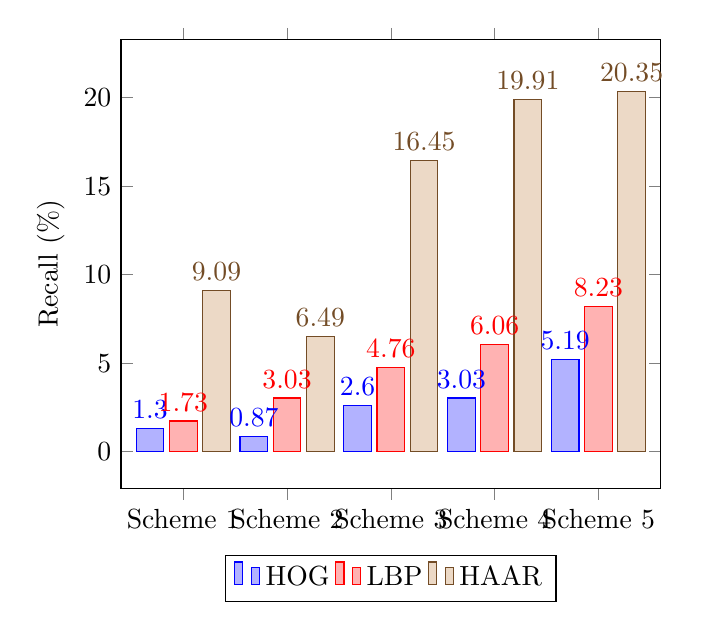
\begin{tikzpicture}
				\begin{axis}[
				    ybar,
				    enlargelimits=0.15,
				    legend style={at={(0.5,-0.15)},
				      anchor=north,legend columns=-1},
				    ylabel={Recall (\%)},
				    symbolic x coords={Scheme 1, Scheme 2, Scheme 3, Scheme 4, Scheme 5},
				    xtick=data,
				    nodes near coords,
				    nodes near coords align={vertical},
				    ]
				\addplot coordinates {(Scheme 1, 1.2987013) (Scheme 2, 0.8658009) (Scheme 3, 2.59740260) (Scheme 4, 3.03030300) (Scheme 5, 5.19480520)};
				\addplot coordinates {(Scheme 1, 1.7316017) (Scheme 2, 3.0303030) (Scheme 3, 4.76190480) (Scheme 4, 6.06060610) (Scheme 5, 8.22510820)};
				\addplot coordinates {(Scheme 1, 9.0909091) (Scheme 2, 6.4935065) (Scheme 3, 16.4502165) (Scheme 4, 19.9134199) (Scheme 5, 20.3463203)};
				\legend{HOG,LBP,HAAR}
				\end{axis}
			\end{tikzpicture}
			\caption{Trial comparison chart.}
			\label{fig:trial_comparison_chart}
		\end{figure}

	}

	\section{Conclusion} {
	\label{sec:conclusion}

		\begin{itemize}
			\item Haar features performed better than HOGS or LBP.
			\item LBP features performed better than HOGS.
			\item Increasing the proportion of negative images decreased the hit rate.
		\end{itemize}

		Image preprocessing techniques future work.

	}

	\bibliographystyle{splncsnat}
	\bibliography{references}

\end{document}
